%%% This part is only that you can run the script alone, please do not change anything here! If you need a special package, add it under the item "extra packages". There is also not layout yet. So don't wonder if it looks bad ;) And it is still without references, I know  %%%

\documentclass[captions=tableheading,twoside]{scrbook}
%% KOMA setup
\setkomafont{caption}{\small}
\setkomafont{captionlabel}{\normalfont\bfseries}
\addtokomafont{sectioning}{\rmfamily}
\setcapindent{1em}

%% Defines look of headers and footers
\usepackage{scrpage2}
	\pagestyle{scrheadings}
	\cofoot[\thepage]{\thepage}
	\cefoot[\thepage]{\thepage}
	\rofoot[]{}
	\lefoot[]{}
	\setheadsepline{.4pt}

%% Costum commands:
	%Command for \agfauthor:
	\newcommand{\agfauthor}[1]{%
	\begin{center}by #1\end{center}}
	\newenvironment{Abstract}{\begin{center}\textbf{Abstract}\end{center}%
	\begin{quote}}{\end{quote}}

	%Command for \vek :
	\newcommand{\vek}[1]{\ensuremath{\boldsymbol{#1}}}

%% Packages:
\usepackage[utf8]{inputenc} % encoding of input
\usepackage[british]{babel} % Language
\usepackage{microtype}
\usepackage{mathtools}  % loads amsmath
	\mathtoolsset{showmanualtags}
\usepackage{bm} % for \bm command --- bold math
\usepackage{float}
\usepackage[farskip=3pt,captionskip=2pt,margin=1em]{subfig}
\usepackage{booktabs,fixltx2e,tabularx,array}
\usepackage{graphicx,epstopdf}

\usepackage{hyperref}          % creates clickable links of refs
\hypersetup{colorlinks=true,
linkcolor=red}

%%% Please insert all extra packages you need here:
%\usepackage{natbib}
% \usepackage{cite}
% \usepackage[round]{natbib}
% \usepackage[]

\usepackage[style=authoryear,
            bibstyle=authoryear,
            backend=biber,
            % refsection=chapter,
            maxbibnames=99,
            maxnames=2,
            firstinits=true,
            uniquename=init,
            natbib=true,
            dashed=false]{biblatex}
\bibliography{bib}





%%%%%%%%%% Start of Document %%%%%%%%%
\begin{document}

\chapter{Report}
\agfauthor{Gullik Vetvik Killie, \large{Add yourself}}

\begin{Abstract}
	Lorem ipsum dolor sit amet, consectetur adipisicing elit, sed do eiusmod
	tempor incididunt ut labore et dolore magna aliqua. Ut enim ad minim veniam,
	quis nostrud exercitation ullamco laboris nisi ut aliquip ex ea commodo consequat.
 	Duis aute irure dolor in reprehenderit in voluptate velit esse cillum dolore eu
	fugiat nulla pariatur. Excepteur sint occaecat cupidatat non proident, sunt in
	culpa qui officia deserunt mollit anim id est laborum.
\end{Abstract}

\section{Introduction}

% Langmuir probes, as well as other instruments, are often situated outside of space crafts.
% The precence of the spacecraft causes disturbances to the local conditions we want to measure,
% these disturbances need to be corrected for.
% Many studies has been done on the flow of plasma around spacecraft and of the wake the
% spacecraft creates \citep{miloch_wake_2010,engwall_wake_2006}.

A spacecraft in space will always be affected by its environment, resulting in various
impacts depending on the orbit (location), types of materials as well as the environment
condition that changes over time \citep{trove.nla.gov.au/work/21680840}. The  most common phenomena on the spacecraft is the so
called charging. The level of charging depends on the energy of particles interacting with
the spacecraft. At lower levels of energy, the form of interaction of charged particles with the
spacecraft only affect the surface part called surface charging. However, for higher levels of energy
worse affects might occur, and in this case the charged particles
can penetrate deep inside the spacecrafts components resulting in so called internal charging \citep{fennell2001spacecraft}.

Charging on the spacecraft can be simulated numerically. Numerous codes have been developed
to explain the behavior of particles around the spacecraft as well as their interactions.
Nevertheless, there still remains many questions since the numerical simulations are only approximations
of real conditions. Although the numerical approach has given good solutions to various applications
such as spaceflight missions. Efforts are made to prove the reliability of a well before launch into space.
One of these efforts is simulating the environment where the satellite will be placed during its mission.
Many parameters are taken into account with respect to its effect on the spacecraft.
The results of the simulations can be a significant point in the decisions made for the spaceflight
mission. This is one of reasons why numerical methods are the primary interest for this study.

In this study, we attempt to simulate a spacecraft named Norsat-1 which will be placed in
Low Earth Orbit (LEO) environment around \(600\) km altitude and polar inclination around \(98.8^\circ\).
This spacecraft is planned to launch in \(2017\)\citep{norSat}. Our simulation was of a smaller spacecraft with dimensions
\(10,10,10\)cm.
This satellite
has been equipped with two probes. It is interesting since this satellite will pass over
the auroral region more frequently. In this region  the satellite will be exposed not only to
rapid variation of the thermal component of the ionosphere \citep{hastings1995review}, but also to high
energy particles from the solar wind, large changes in the direction of the magnetic field, etc.

Since we use the EMSES (Electro Magnetic Spacecraft Environment Simulator) code \citep{miyake_plasma_2013} in the
simulation, it is important to point out that only the effects of background plasma as
well as the photoelectrons from the sunlight are taken into account. The simulations
are done in several cases and each case has been grouped into two, i.e. plasma
flows with and without the photoemission effects on the spacecraft as well as the probes.
All results will be presented in detail in the specific section in this report.


\section{Theory}
\input{theory}

\section{Numerical Methods}
\subsection{Numerical methods}

To solve the problem numerically we use the EMSES code. EMSES uses the standard PIC method for plasma simulations \citep{birdsall2004plasma}.
In the code we are able to define a spacecraft body, and the code then calculates the potential on that body using the capacitance matrix method.
Although EMSES has the capability to do a full electromagnetic calculation, we have opted to use the Poisson's equation
solver for electrostatic problems. In the EMSES system we can define sunlit surfaces based upon an angle, and a current
density. Sunlit surfaces will then emit electrons based upon a energy distribution. For a complete description of EMSES' capabilities
see \citep{nakashima_ohhelp:_2009}. Parameters are choosen to simulate the sun at the earth, but with an enhanced flux to emphasize the effect in question.

\subsection{Theoretical calculations}
\label{sec:theo_calc}

If there are big difference between spacecraft size and the Debye length of plasma, we can evaluate the theoretical potential of the spacecraft($\Phi_d$). In order to get $\Phi_d$, we need the ion, electron and photoelectron current (\(I_i\), \(I_e\) and \(I_{ph}\)).\\
In the case that the value of $\Phi_d$ is considered to be negative, each current is written as below:

\begin{equation}
\begin{split}
 I_i = &
    \left\{\begin{array}{ccc}
       A|q|n_\infty\sqrt{\frac{8 k T_i}{\pi m_i}} (without flow)\\
       \frac{1}{6}A |q|n_\infty V + \frac{5}{6} A |q| n_\infty \sqrt{\frac{8 k T_i}{\pi M_i}}(with flow)
      \end{array}\right. \\
  I_e = & -A|q|n_\infty \sqrt{\frac{8 k T_e}{\pi m_e}}exp\Big(\frac{|q|\Phi_d}{k T_e}\Big)\\
  I_{ph} = & \frac{1}{6} AJ_s
\end{split}
\label{thin sheet potential}
\end{equation}
where \(A\) is the surface area of the spacecraft, \(|q|\) is elementary charge, \(n_\infty\) is the plasma density, \(k\) is Boltzmann's constant, \(T_i\)/\(T_e\) is the temperature of ion/electron, \(M_i\)/\(M_e\) is the mass of ion/electron and \(J_s\) is the photoelectron density.
Submitting these equations to \(I_i+I_e+I_{ph}=0\) and solving for $\Phi_d$, we can get
\begin{equation}
\begin{split}
 \Phi_d = & \frac{k T_e}{|q|}ln\Big(\sqrt{\frac{T_i}{T_e}}\sqrt{\frac{m_e}{m_i}}+\frac{J_s}{6 n_\infty |q|}\sqrt{\frac{\pi m_e}{8 k T_e}}\Big) + \Phi_0 \\
 \Phi_d = & \frac{k T_e}{|q|}ln\Big(\frac{5}{6}\sqrt{\frac{T_i}{T_e}}\sqrt{\frac{m_e}{m_i}}+\frac{V}{6}\sqrt{\frac{\pi m_e}{8 k T_e}} + \frac{J_s}{6 n_\infty |q|}\sqrt{\frac{\pi m_e}{8 k T_e}} \Big)+\Phi_0 \\
 \Phi_0 = & k T_{ph}, \ V = speed\ of\ flow
\end{split}
\label{thin sheet potential 2}
\end{equation}
where \(T_{ph}\) is the temperature of photoelectron.
The theory is based on thin-sheath approximation, so if spacecraft size is much larger than the Debye length of plasma, we can use it.\\

\subsection{Test case setup}

We wish to simulate the effects of Photon emitted electrons in different test cases, and have thus set up the following
6 cases:
\begin{table}
\begin{center}
    \begin{tabular}{ | l | l | l | p{5cm} |}
    \hline
    Case & Plasma flow (\(V\)) & Photon emission  \\ \hline
     1: & 41600 $\vec{e_x}$ m/s  & 0 \\ \hline
     2: & -41600 $\vec{e_z}$ m/s & 0 \\ \hline
     3: & -41600 $\vec{e_y}$ m/s & 0 \\ \hline
     4: & 41600 $\vec{e_x}$ m/s & $-10^{-3} A/m^{3}$ $\vec{e_x}$\\ \hline
     5: & -41600 $\vec{e_z}$ m/s & $-10^{-3} A/m^{3}$ $\vec{e_x}$\\ \hline
     6: & -41600 $\vec{e_y}$ m/s & $-10^{-3} A/m^{3}$  $\vec{e_x}$\\
    \hline
    \end{tabular}
\end{center}
	\caption{The six different cases we investigate, \(1-3\) is without a photoemission, and \(4-6\) is the same cases with photoemission.}
\end{table}

	\begin{table}[h]
		\centering
	    \begin{tabular}{ | l | l | l| l| l | l | l |}
	    \hline
		Stepsize & Timestep & Density &\(|B|\) & \(T_e\) & \(T_i\) & N\(_x\)\\
		\hline
		\(1.0\)cm & \(5\text{E}-10\)s & \(1.0\text{E}5\)kg/cm\(^3\) &  \(50\text{E}-6\) T & \(3000\)K & \(1500\)K  & \(128\)\\
	    \hline
	    \end{tabular}
		\caption{Input parameters in EMSES}
	\end{table}

So test case 1-4, 2-5, and 3-6 are the ``same'' cases except that we run the simulation with and without
photon emission to compare the cases two and two. We define 3 geometric objects, the spacecraft itself
and two probes. In all cases the $B$ field is in the $\vec e_z$ direction.

\begin{figure}
        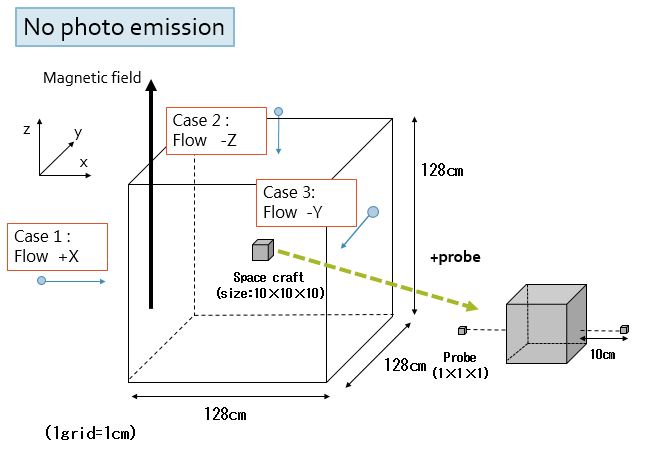
\includegraphics[width = \textwidth]{images/picture_simulation1.png}
	\caption{(a)Geometry of spacecraft and surroundings. Figure is no P-E simulation cases.}
        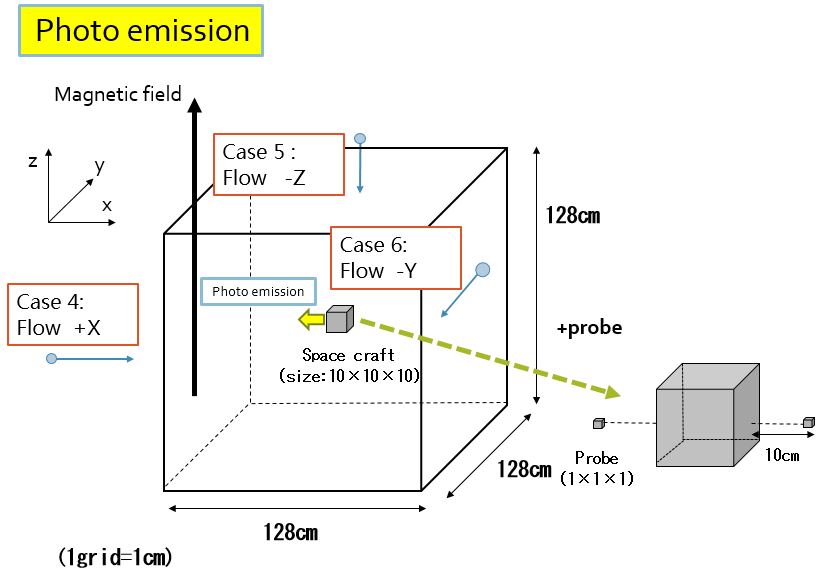
\includegraphics[width = \textwidth]{images/picture_simulation2-2.png}
        \caption{(b)Geometry of spacecraft and surroundings. Figure is P-E simulation cases.}
    \end{figure}


\section{Results}
\subsection{Induced electric current}
	%Redo this part if necessary
	The plasma is flowing in in relation to the coordinate system in the simulations.
	Due to this an induced electrical field, \(\varepsilon\), will appear.
	The induced electrical field will neutralize the Lorentz force.
	Combined with the electrostatic approximation we can obtain the \(\varepsilon\)

	\begin{equation}
		\vec{\varepsilon} = \vec{v_D}\times \vec{B}
	\end{equation}

	This will cause a potential gradient perpendicular to the plasma flow and the magnetic field,
	using the electrostatic approximation we obtain the magnitude of the gradient.

	\begin{equation}
		\int{Edx} = -\phi
	\end{equation}

	\begin{equation}
		\phi = -\int \vec{v}_d\times\vec{B} \approx -\int \left( 41600 \text{m/s}\cdot 50E-6 \text{T} \right) dx
	\end{equation}
	\begin{equation}
		|\nabla\phi| = 2.08 \text{m}^{-1}
	\end{equation}

	\begin{figure}
		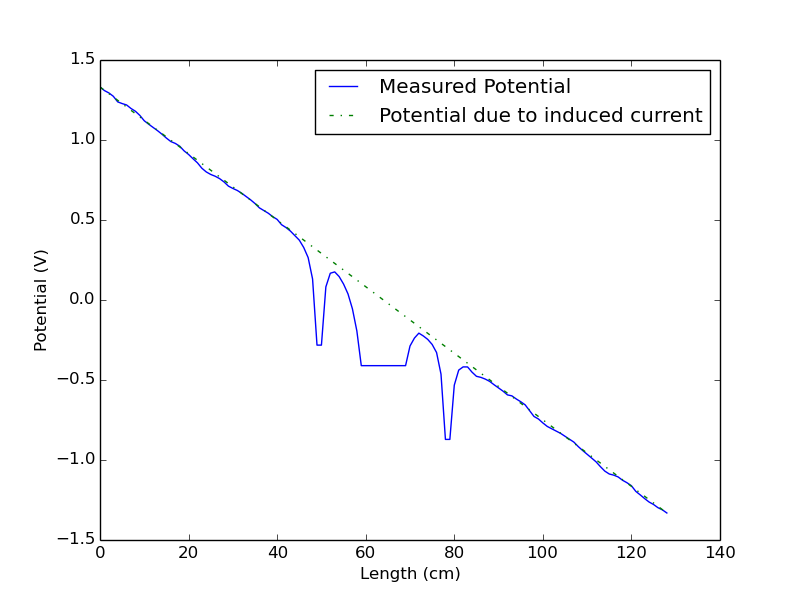
\includegraphics[width = \textwidth]{images/emph}
		\caption{The blue line is the potential along direction x for simulation \(6\). In this case the potential gradient is along
		the \(x-\)axis. The dotted green line is the potential caused by the induced electrical field. This should be accounted for
		if  we want to find the potential at the spacecraft and the probes.}
		\label{fig:emph}
	\end{figure}

	Figure~\ref{fig:emph} shows the measured potential at case \(6\).

\subsection{Photoemmision paths}

	The electrons emmited from the spacecraft due to the photoelectric effect, have a kinetic
	energy corresponding to a Maxwellian distribution with a temperature of \(T_{ph} =  3.8481\cdot 10^{4} \text{K}\).
	Figure~\ref{fig:trajectories} illustrates the trajectories of the emmited electrons in simulation \(6\).
	As the probes are situated \(10 \text{cm}\) to the sides of the spacecraft on the \(x-\)axis, the probes
	may be hit by the photo-emmited electrons. In the following section, \ref{sec:acc_emmited}, we show the number of electrons hitting
	the probes.


	\begin{figure}
		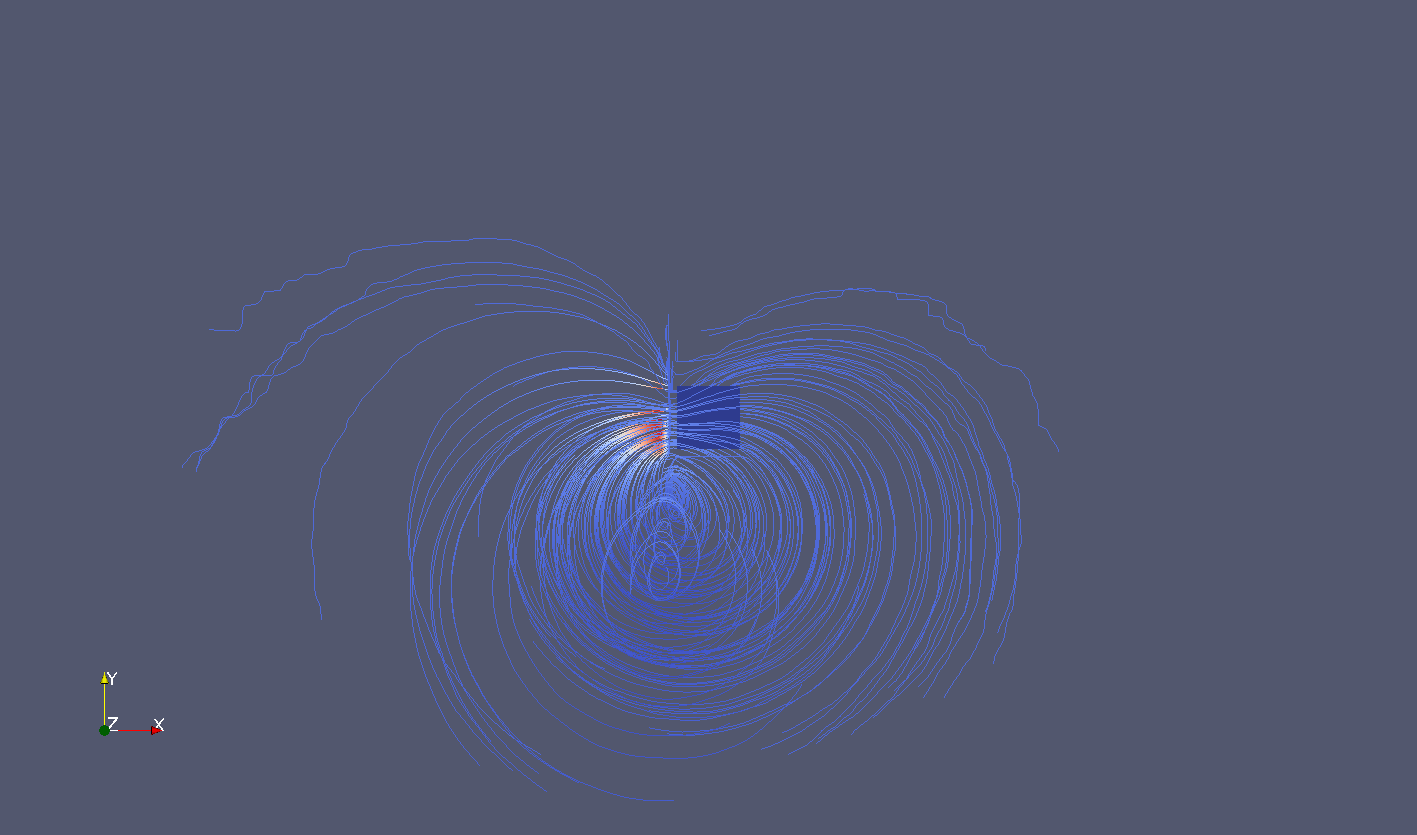
\includegraphics[width = 0.49 \textwidth]{images/case6_jph_paths}
		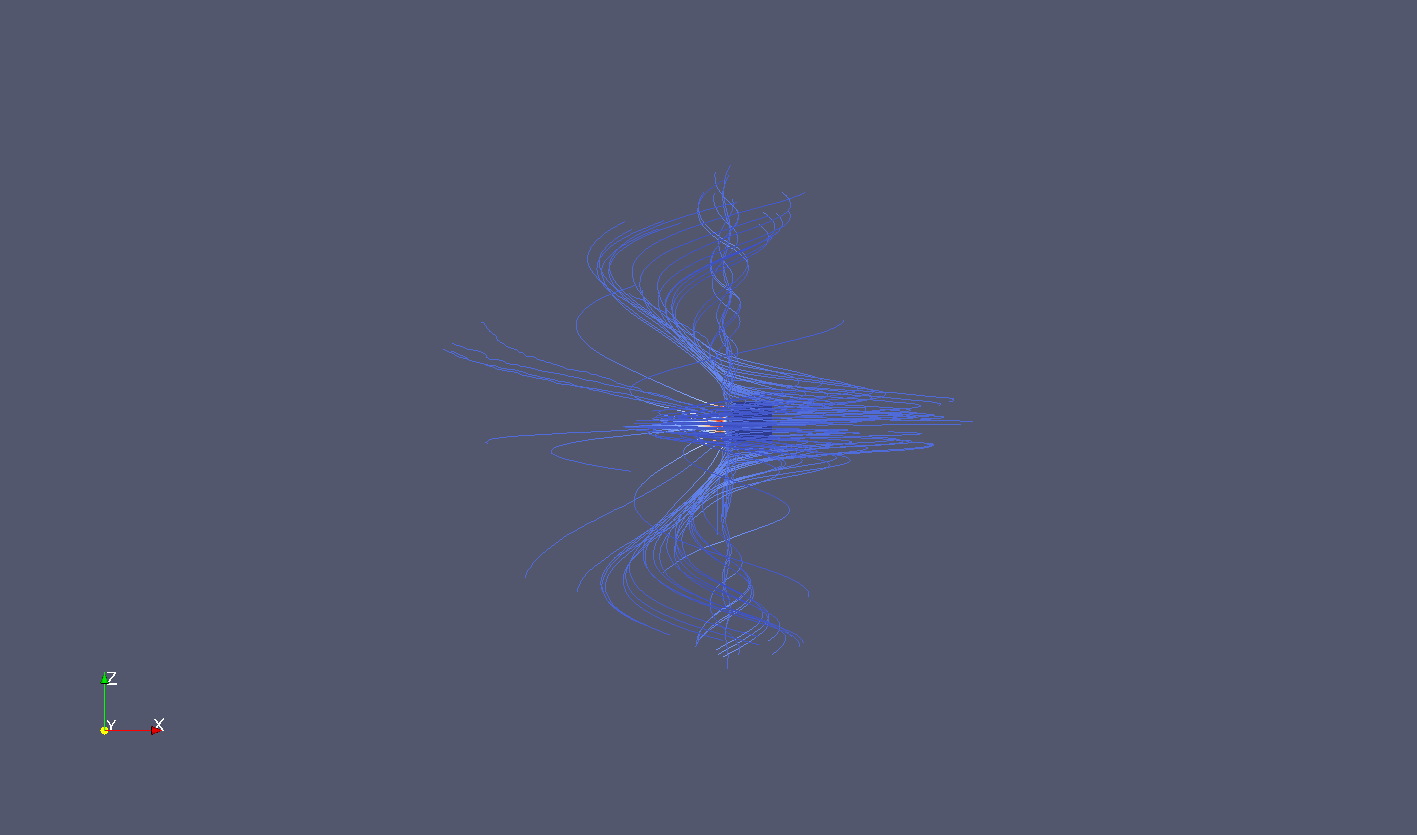
\includegraphics[width = 0.49 \textwidth]{images/case6_jph_paths_2}
		\caption{The trajectories of the electrons emmited by the photoelectric effect in simulation \(6\). The possible
		paths of the photoemmited electrons coincide with the volume occupied by the langmuir probes. The photoemmited electrons are strongly affected by the magnetic
		field \(\vec{B}\), and follows a gyrating path guided by \(\vec{B}\). The photoemmited electrons are in all the studied cases
		emmited from the spacecraft in \(-x\) direction, and the paths are similar. The langmuir probes are situated \(10 \text{cm}\) to each side
		of the spacecraft along the \(x-\)direction. (NOTE, should have axis labels, and domain length.)}
		\label{fig:trajectories}
	\end{figure}

\subsection{Accumulated Photoelectrons on Langmuir Probes}

In the simulations both electrons and photoelectrons are absorbed by the probes. Table~\ref{tab:elec_current} shows the current
of both regular electrons, as well as photoelectrons, interacting with the probes.
The photoelectrons are emmited on the left side of the spacecraft and we see a larger current of
photoelectrons here. The current caused by the photoemmision is \(10-100\) smaller than the current
from the electrons in the plasma.

\begin{figure}[h]
	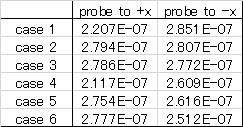
\includegraphics[width = 0.45\textwidth]{images/caliculation_of_electron_current}
	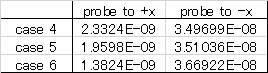
\includegraphics[width = 0.45\textwidth]{images/caliculation_of_PE_current}
	\caption{The left table shows the electron current hitting the inserted probes at
	for the simulated cases \(1-6\). On the table to the right the photoelectrons hitting the probes are shown.
	The photoelectron current is smaller than the electron current from the plasma, varying from \(10-100\) times smaller.}
	\label{tab:elec_current}
\end{figure}

\subsection{Potential difference with P-E and no P-E}

\subsubsection{Case 1 vs case 4}

\begin{figure}
    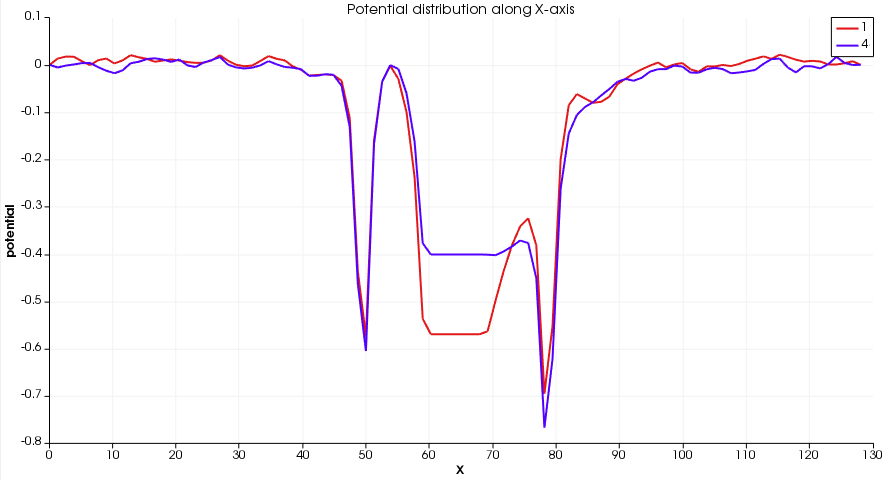
\includegraphics[width = 0.3 \textwidth]{images/pot_case14.png}
    \caption{Potential of satelite and surroundings in the x-direction for case 1 and case4. Note that the potential drop i much greater in the right probe when comparing the two cases.}
\end{figure}


In case 4 we have the emitted electrons in the negative flow direction. As expected this
leads to a drop in potential in the left probe which is facing the plasma flow. The
potential drop over the probe is 0.02V or 3.8\%. The right probe is now the wake where we have
a drop in the ion density. This yields a large drop in potential compared to the left
probe, but it also has a larger potential drop than the left probe when comparing case 1 and 4. This
might be because the increase in electron density on the left side redirects more ions from the right side.
The potential drop in the right probe comparing the two cases is 0.07V or 10\%. The potential rise over the satelite is 0.17V or 28\%.


\subsubsection{Case 2 vs case 5}


\begin{figure}
    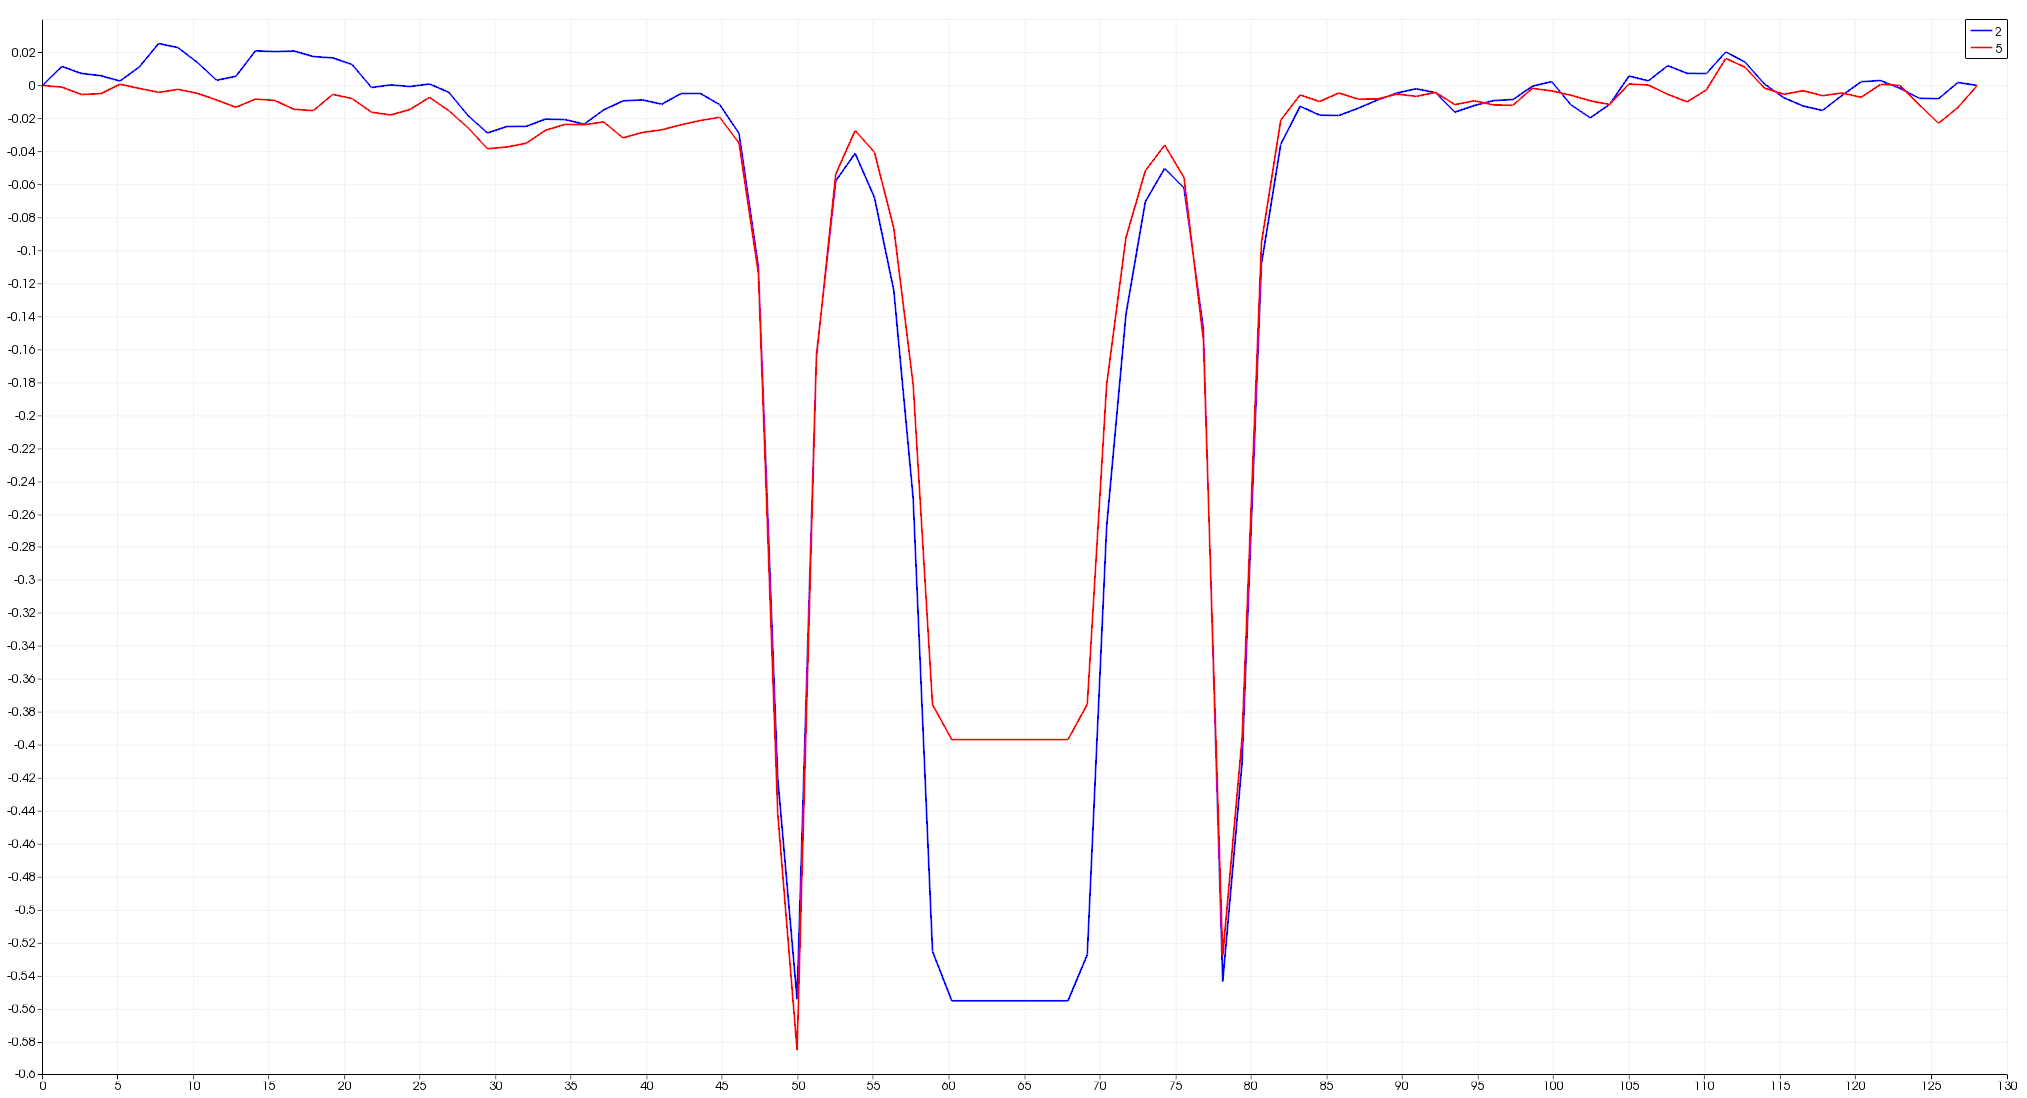
\includegraphics[width = 0.5 \textwidth]{images/pot_case25.png}
    \caption{Figure show potential of satelite and surroundings in the x-direction for case 2 and 5. Note that we have a small potential drop in the left probe but a potential rise in the right probe when comparing the two cases.}
    \label{fig:pot_case25}
\end{figure}

With the flow of emmited electrons in the negative x direction we would expect a rise in electron density around the left probe.
This can be seen in figure \ref{fig:pot_case25} where we see a potential drop of 0.03V or 5.4\% over this probe compared to case 5 with no emitted
electrons. On the right probe we have a small rise in the potential of 0.018V or 3.3\%. With no emitted electrons on this side of the satelite the rise in
potential can be explained by looking at the increase in ion density as seen in figure (need ref).
In the satelite we have a potential rise of 0.16V or 28\%. So the potential change in the probes are small compared to the potential change in the satelite.

\subsubsection{Case 3 vs case 6}

\begin{figure}
    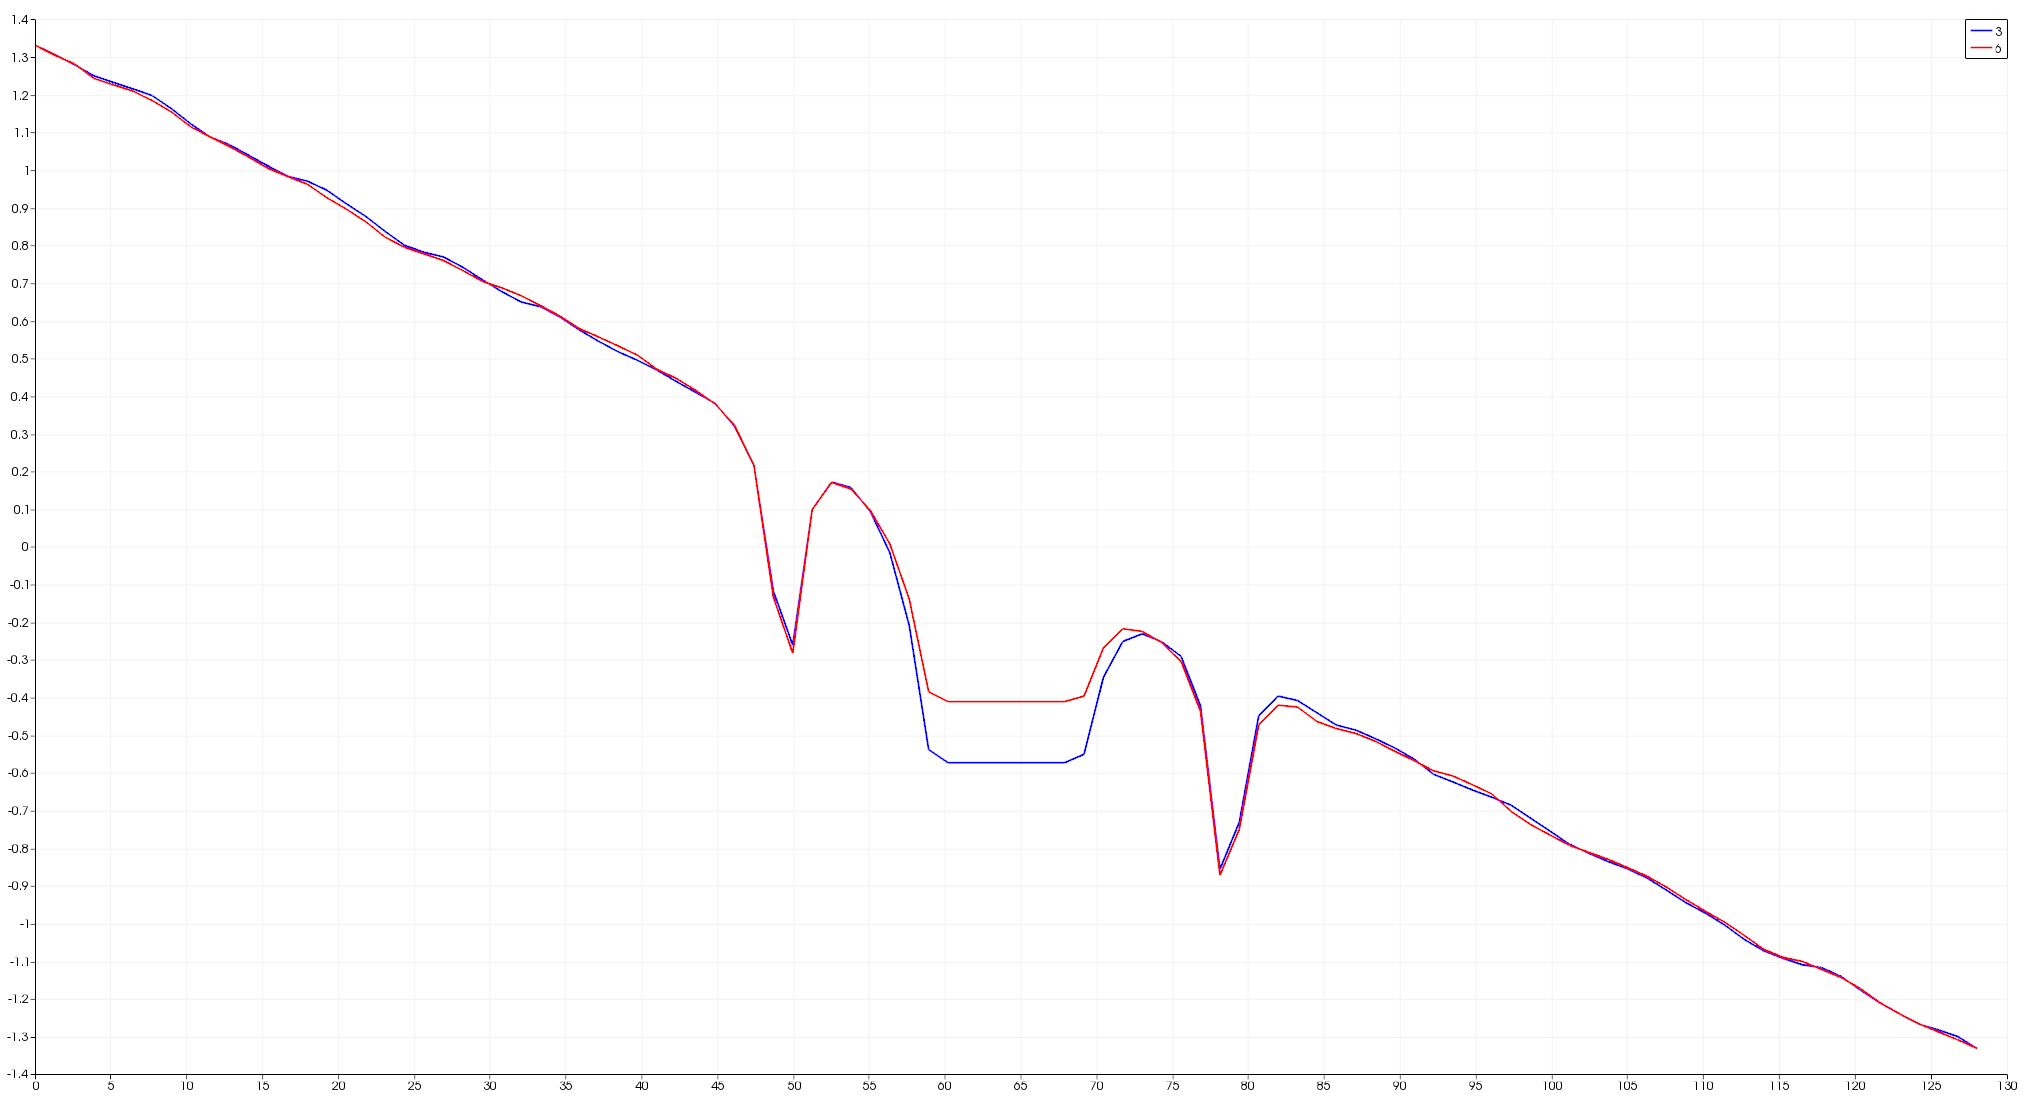
\includegraphics[width = 0.5 \textwidth]{images/pot_case36.png}
    \caption{Figure show potential of satelite and surroundings in the x-direction for case 3 and 6. Note that there is almost the same drop in potential for both probes.}
\end{figure}

Here we have almost the same drop in potential over both probes of about 0.03V. However this change yields 12\% for the left probe but only 3\% for the right probe. Over the satelite we have a potential rise of 0.15V which yields a 26\% change.

\subsection{Wake plots}
	The spacecraft is moving relative to the plasma flow, this causes a wake to be formed in the vicinity of the craft.
 	Figures~\ref{fig:wake} illustrates the flow in case \(1,2\) and \(3\).

    \begin{figure}
        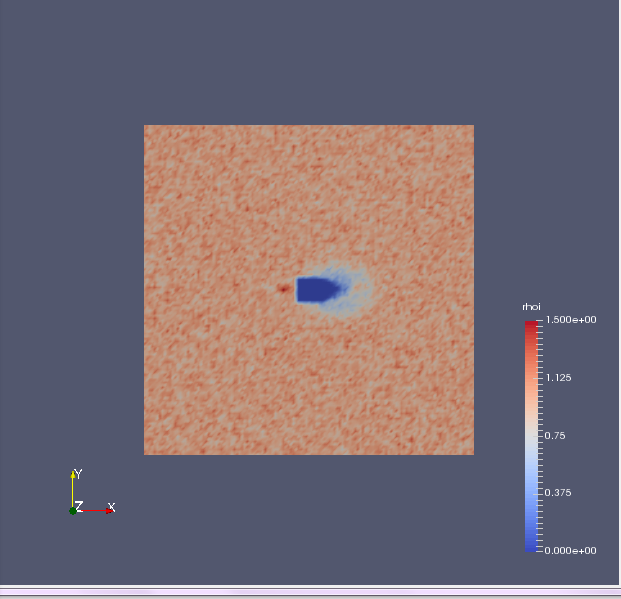
\includegraphics[width = 0.3 \textwidth]{images/ion_density_case1}
        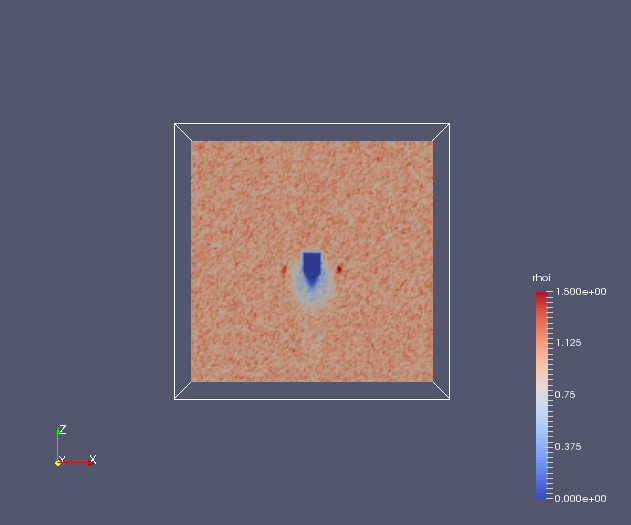
\includegraphics[width = 0.3 \textwidth]{images/ion_density_x-z_case2}
	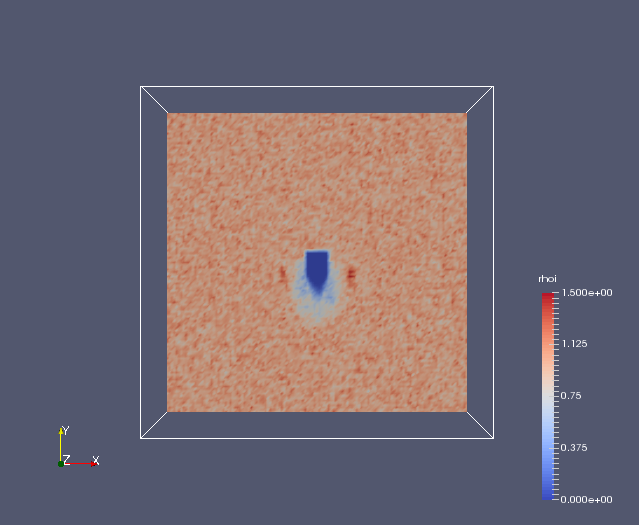
\includegraphics[width = 0.3 \textwidth]{images/ion_density_x-y_case3}
        \caption{Ion density of spacecraft and surroundings without P-E. Figure on the left displays case 1. Middle figure displays case 2. Rightmost figure displays case 3.}
		\label{fig:wake}
    \end{figure}


\section{Discussion}


We compared P-E and without P-E. We think whether photo emission affect the Probes.
We set the size of the Probes to 1 $cm^3$ in this simulation. But it is the same size as the grid. So density does not become 0 in the inner of Probes. We need to simulate a variety of sizes. We try the case of more number of grid, longer a grid, and size of Probes.
In order to measure the characteristic value of each particle, we set probes in the place that the wake is formed or not. But they are not a real physical model. (For example, if we give probes the photoelectric effect or if we change the size of satellite and probes to realistic scales, the results might be changed.)
We see a difference in cases, so it might be a case we have not considered that that is significant.



\section{Conclusions}

In the LEO regime, where the simulations have been done, the photoemmited currents are weak compared with
background plasma. Because of this the effect seen on the Langmuir probes were small, further studies should be done
in other plasma regimes where the photoemmision is more pronounced, i.e. MEO, GEO or in the magnetospheric tail lobes.



\nocite{*}
% \bibliographystyle{plainnat}
% \printbibliography



\end{document}

%%% Local Variables:
%%% mode: latex
%%% mode: auto-fill
%%% mode: flyspell
%%% eval: (ispell-change-dictionary "english")
%%% TeX-master: "../AGF212_ReportSpring2013"
%%% End:
